\section{Datenbanken}
\label{sec:Datenbanken}

IHK Belegsatz \cite{IHKBelegsatz}

\begin{center}
	\setlength\arrayrulewidth{1pt}
	\begin{tabular}{|p{0.45\textwidth} | p{0.55\textwidth}|}
		\hline
		\textbf{Syntax} & \textbf{Beschreibung} \\
		\hline
		\rowcolor{tableLightGray} \textit{Tabelle} &  \\
		\hline
		\begin{tabular}[t]{l}
			\textbf{CREATE TABLE} Tabellenname(\\ Spaltenname <DATENTYP>,\\ Primärschlüssel,\\ Fremdschlüssel)
		\end{tabular} & Erzeugt eine neue leere Tabelle mit der beschriebenen Struktur \\
		\hline
		\begin{tabular}[t]{l}
			\textbf{ALTER TABLE} Tabellenname\\ \hspace{.5em} \textbf{ADD COLUMN} Spaltenname Datentyp\\ \hspace{.5em} \textbf{DROP COLUMN} Spaltenname Datentyp\\ \\ \textbf{ADD FOREIGN KEY}(Spaltenname)\\ \hspace{1em} \textbf{REFERENCES} Tabellenname(\\ \hspace{8em} Primärschlüssel) \\
		\end{tabular} & 
		\begin{tabular}[t]{l}
			Änderungen an einer Tabelle:\\
			\hspace{1em}Hinzufügen einer Spalte\\
			\hspace{1em}Entfernen einer Spalte\\\\
			\hspace{1em}Definiert eine Spalte als Fremdschlüssel
		\end{tabular}\\
		\hline
		\textbf{CHARACTER} & Textdatentyp \\
		\hline
		\textbf{DECIMAL} & Numerischer Datentyp (Festkommazahl)\\
		\hline
		\textbf{DOUBLE} & Numerischer Datentyp (Doppelte Präzision)\\
		\hline
		\textbf{INTEGER} & Numerischer Datentyp (Ganzzahl)\\
		\hline
		\textbf{DATE} & Datum (Format DD.MM.YYYY)\\
		\hline
		\textbf{PRIMARY KEY} (Spaltenname) & Erstellung eines Primärschlüssels \\
		\hline
		\begin{tabular}[t]{l}
			\textbf{FOREIGN KEY} (Spaltenname)\\
			\hspace{1em} \textbf{REFERENCES} Tabellenname(\\
			\hspace{2em}Primärschlüsselspaltenname)
		\end{tabular} & Erstellung einer Fremdschlüssel-Beziehung\\
		\hline
		\textbf{DROP TABLE} Tabellenname & Löscht eine Tabelle\\
		\hline
		\rowcolor{tableLightGray} \textit{Befehle, Klauseln, Attribute} & \\
		\hline
		\textbf{SELECT *} | Spaltenname1 [, Spaltenname2, ...] & Wählt die Spalten einer oder mehrerer Tabellen, deren Inhalte in die Liste aufgenommen werden sollen; alle Spalten (*) oder die namentlich aufgeführten\\
		\hline
		\textbf{FROM} & Name der Tabelle oder Namen der Tabellen, aus denen die Daten der Ausgabe stammen sollen\\
		\hline
		\begin{tabular}[t]{l}
			\textbf{SELECT ...}\\
			\textbf{FROM ...}\\
			\hspace{1em}\textbf{(SELECT ...}\\
			\hspace{1em}\textbf{FROM ...}\\
			\hspace{1em}\textbf{WHERE ...) AS} tbl\\
			\textbf{WHERE ...}
		\end{tabular} & Unterabfrage (subquery), die in eine äußere Abfrage eingebettet ist. Das Ergebnis der Unterabfrage wird wie eine Tabelle - hier mit Namen "tbl" - behandelt. \\
		\hline
	\end{tabular}
\end{center}

\begin{center}
	\setlength\arrayrulewidth{1pt}
	\begin{tabular}{|p{0.45\textwidth} | p{0.55\textwidth}|}
		\hline
		SELECT \textbf{DISTINCT} & Eliminiert Redundanzen, die in einer Tabelle auftreten können. Werte werden jeweils nur einmal angezeigt.\\
		\hline
		\textbf{JOIN / INNER JOIN} & Liefert nur die Datensätze zweier Tabellen, die gleiche Datenwerte enthalten\\
		\hline
		\textbf{LEFT JOIN / LEFT OUTER JOIN} & Liefert von der erstgenannten (linken) Tabelle alle Datensätze und von der zweiten Tabelle jene, deren Datenwerte mit denen der ersten Tabelle übereinstimmen\\
		\hline
		\textbf{RIGHT JOIN / RIGHT OUTER JOIN} & Liefert von der zweiten (rechten) Tabelle alle Datensätze und von der ersten Tabelle jene, deren Datenwerte mit denen der zweiten Tabelle übereinstimmen\\
		\hline
		\textbf{WHERE} & Bedingung, nach der Datensätze ausgewählt werden sollen\\
		\hline
		\begin{tabular}[t]{l}
			\textbf{WHERE EXISTS} (subquery)\\
			\textbf{WHERE NOT EXISTS} (subquery)
		\end{tabular} & Die Bedingung EXISTS prüft, ob die Suchbedingung einer Unterabfrage mindestens eine Zeile zurückliefert. NO EXISTS negiert die Bedingung.\\
		\hline
		\begin{tabular}[t]{l}
			\textbf{WHERE ... IN} (subquery)\\\\
			\textbf{WHERE NOT ... IN} (subquery)
		\end{tabular} & 
		\begin{tabular}[t]{l}
			Der Wert des Datenfelds ist in der ausgewählten Menge \\vorhanden.\\
			Der Wert des Datenfelds ist in der ausgewählten Menge \\nicht vorhanden.
		\end{tabular}\\
		\hline
		\textbf{GROUP BY} Spaltenname1 [, Spaltenname2, ...] & Gruppierung (Aggregation) nach Inhalt des genannten Feldes\\
		\hline
		\textbf{ORDER BY} Spaltenname1 [, Spaltenname2, ...] \textbf{ASC | DESC} & Sortierung nach Inhalt des genannten Feldes oder der genannten Felder ASC: aufsteigend; DESC: absteigend\\
		\hline
		\rowcolor{tableLightGray} \textit{Datenmanipulation} & \\
		\hline
		\textbf{DELETE FROM} Tabellenname & Löschen von Datensätzen in der genannten Tabelle\\
		\hline
		\textbf{UPDATE} Tabellenname \textbf{SET} & Aktualisiert Daten in Feldern einer Tabelle\\
		\hline
		\begin{tabular}[t]{l}
			\textbf{INSERT INTO} Tabellenname\\
			\hspace{8em}[(spalte1, spalte2, ...)]\\
			\hspace{1em}\textbf{VALUES} (Wert Spalte 1 \\
			\hspace{8em}[, Wert Spalte 2, ...])\\
			oder\\
			\hspace{1em}\textbf{SELECT ... FROM ... WHERE}
		\end{tabular} & Fügt Datensätze in die genannte Tabelle ein, die entweder mit festen Werten belegt oder Ergebnis eines SELECT-Befehls sind\\
		\hline
		\rowcolor{tableLightGray} \textit{Berechtigungen kontrollieren} & \\
		\hline
		\textbf{CREATE} Benutzer | Rolle \textbf{IDENTIFIED BY} 'Passwort' & Erzeugt einen neune Benutzer oder eine neue Rolle mit einem Passwort\\
		\hline		
		\begin{tabular}[t]{l}
			\textbf{GRANT} Recht | Rolle \textbf{ON} *.* | Datenbank.* | \\
			Datenbank.Objekt\\
			\textbf{TO} Benutzer | Rolle [WITH GRANT OPTION]
		\end{tabular} & 
		\begin{tabular}[t]{l}
			Weist einem Benutzer oder einer Rolle ein Recht auf ein \\
			bestimmtes Datenbank-Objekt\\
			Weist einem Benutzer eine Rolle zu
		\end{tabular}\\
		\hline
		\begin{tabular}[t]{l}
			\textbf{REVOKE} Recht | Rolle \textbf{ON} *.* | Datenbank.* | \\
			Datenbank.Objekt\\
			\textbf{FROM} Benutzer | Rolle
		\end{tabular} & 
		\begin{tabular}[t]{l}
			Entzieht einem Benutzer oder einer Rolle ein Recht auf ein \\
			bestimmtes Datenbank-Objekt\\
			Entzieht einem Benutzer eine Rolle
		\end{tabular}\\
		\hline
	\end{tabular}
\end{center}

\begin{center}
	\setlength\arrayrulewidth{1pt}
	\begin{tabular}{|p{0.45\textwidth} | p{0.55\textwidth}|}
		\hline
		\rowcolor{tableLightGray} \textit{Aggregatfunktionen} & \\
		\hline
		\textbf{AVG} (Spaltenname) & Ermittelt das arithmetische Mittel aller Werte im angegebenen Feld\\
		\hline
		\textbf{COUNT} (Spaltenname | *) & Ermittelt die Anzahl der Datensätze mit Nicht-NULL-Werten im angegebenen Feld oder alle Datensätze der Tabelle (dann mit Operator *)\\
		\hline
		\textbf{SUM} (Spaltenname | Formel) & Ermittelt die Summe aller Werte im angegebenen Feld oder der Formelergebnisse\\
		\hline
		\textbf{MIN} (Spaltenname | Formel) & Ermittelt den kleinsten aller Werte im angegebenen Feld\\
		\hline
		\textbf{MAX} (Spaltenname | Formel) & Ermittelt den größten aller Werte im angegebenen Feld\\
		\hline
		\rowcolor{tableLightGray} \textit{Funktionen} & \\
		\hline
		\textbf{LEFT} (Zeichenkette, Anzahlzeichen) & Liefert \textit{Anzahlzeichen} der Zeichenkette von links.\\
		\hline
		\textbf{RIGHT} (Zeichenkette, Anzahlzeichen) & Liefert \textit{Anzahlzeichen} der Zeichenkette von rechts.\\
		\hline
		\textbf{CURRENT} & Liefert das aktuelle Datum mit der aktuellen Uhrzeit\\
		\hline
		\textbf{CONVERT(time,}[DatumZeit]) & Liefert die Uhrzeit aus einer DatumZeit-Angabe\\
		\hline
		\textbf{DATE} (Wert) & Wandelt einen Wert in ein Datum um\\
		\hline
		\textbf{DAY} (Datum) & Liefert den Tag des Monats aus dem angegebenen Datum\\
		\hline
		\textbf{MONTH} (Datum) & Liefert den Monat aus dem angegebenen Datum\\
		\hline
		\textbf{TODAY} & Liefert das aktuelle Datum\\
		\hline
		\textbf{WEEKDAY} (Datum) & Liefert den Tag der Woche aus dem angegebenen Datum\\
		\hline
		\textbf{YEAR} (Datum) & Liefert das Jahr aus dem angegebenen Datum\\
		\hline
		\textbf{DATEADD} (Datumsteil, Intervall, Datum) & Fügt einem Datum ein Intervall (ausgefrückt in den unter Datumsteil angegebenen Einheiten) hinzu\\
		\hline
		\textbf{DATEDIFF} (Datumsteil, Anfangsdatum, Enddatum) Datumsteile: \textbf{DAY, MONTH, YEAR} & Liefert Enddatum-Startdatum (ausgedrückt in den unter Datumsteil angegebenen Einheiten)\\
		\hline
		\rowcolor{tableLightGray} \textit{Operatoren} & \\
		\hline
		\textbf{AND} & Logisches UND\\
		\hline
		\textbf{LIKE} & Überprüfung von Text auf Gleichheit wenn Platzhalter ('regular expressions') eingesetzt werden.\\
		\hline
		\textbf{NOT} & Logische Negation\\
		\hline
		\textbf{OR} & Logisches ODER\\
		\hline
		\textbf{IS NULL} & Überprüfung auf NULL\\
		\hline
		\textbf{=} & Test auf Gleichheit\\
		\hline
		\textbf{>, >=, <, <=, <>} & Test auf Ungleichheit\\
		\hline
		\textbf{*} & Multiplikation\\
		\hline
		\textbf{/} & Division\\
		\hline
		\textbf{+} & Addition, positives Vorzeichen\\
		\hline
		\textbf{-} & Subtraktion, negatives Vorzeigen\\
		\hline
	\end{tabular}
\end{center}


\subsection{Datenbankmodelle und -modellierung}
\label{sec:Datenbankmodelle}

\subsubsection{Relationale und nicht-relationale Datenbanken}
\label{sec:RelationaleDatenbanken}

Eine nicht relationale Datenbank ist eine Datenbank, die nicht das tabellarische Schema mit Zeilen und Spalten verwendet, das in den meisten herkömmlichen Datenbanksystemen zum Einsatz kommt. \hl{Nicht relationale Daten verwenden stattdessen ein Speichermodell, das für die spezifischen Anforderungen des gespeicherten Datentyps optimiert ist}. So können die Daten beispielsweise als einfache \hl{Schlüssel-Wert-Paare}, als \hl{JSON-Dokumente} oder als Diagramm mit Edges und Scheitelpunkten gespeichert werden. \cite{microsoftNichtRelational}

\subsubsection{ERD (Entity-Relationship-Modell)}
\label{sec:ERD}

\begin{center}
	\begin{tikzpicture}[align=center, node distance=1cm]
	\node (entity1) [entity] {Entität 1};
	\node (attribute) [attribute, left=of entity1] {attribut};
	\draw (entity1) -- (attribute);
	\node (relationship) [relationship, right=of entity1] {beziehung};
	\draw (entity1) -- (relationship) node[pos=.3,above]{1};
	\node (entity2) [entity, right=of relationship] {Entität 2};
	\draw (relationship) -- (entity2) node[pos=.7,above]{n};
\end{tikzpicture}
\end{center}

Kardinalitäten:\\

Entitäten besitzen unterschiedliche Kardinalitäten, also die Anzahl zuordenbarer Objekte einer anderen Entität. Es gibt die Ausprägungen 1:1 (eins zu eins), 1:n (eins zu mehreren) und n:m (mehrere zu mehreren). \cite{ERDKardinalitaeten}


\subsubsection{NoSQL}
\label{sec:NoSQL}

NoSQL-Datenbanken wurden speziell für bestimmte Datenmodelle entwickelt und \hl{speichern Daten in flexiblen Schemas}, die sich leicht für moderne Anwendungen skalieren lassen. NoSQL-Datenbanken sind für ihre einfache Entwicklung, Funktionalität und Skalierbarkeit weithin bekannt. \cite{AWSnoSQL}

\paragraph{Flexibilität} NoSQL-Datenbanken bieten in der Regel flexible Schemata, die eine schnellere und iterativere Entwicklung ermöglichen. Das flexible Datenmodell macht NoSQL-Datenbanken ideal für halbstrukturierte und unstrukturierte Daten.

\paragraph{Skalierbarkeit} NoSQL-Datenbanken sind in der Regel so konzipiert, dass sie durch die Verwendung von verteilten Hardware-Clustern skaliert werden können, im Gegensatz zu einer Skalierung durch das Hinzufügen teurer und robuster Server. Einige Cloud-Anbieter übernehmen diese Vorgänge im Hintergrund als vollständig verwaltete Dienstleistung.

\paragraph{Hohe Leistung} NoSQL-Datenbanken sind für bestimmte Datenmodelle und Zugriffsmuster optimiert. Diese ermöglichen eine höhere Leistung, als wenn Sie versuchen würden, ähnliche Funktionen mit relationalen Datenbanken zu erreichen.

\paragraph{Hochfunktionell} NoSQL-Datenbanken bieten hochfunktionelle APIs und Datentypen, die speziell für ihre jeweiligen Datenmodelle entwickelt wurden.

\subsubsection{Welche Arten von NoSQL-Datenbanken gibt es?}
\label{sec:ArtenNoSQL}

\paragraph{Schlüsselwertdatenbanken} Eine Schlüsselwertdatenbank \hl{speichert Daten als eine Sammlung von Schlüsselwertpaaren}, in denen ein Schlüssel als eindeutiger Identifikator dient. Schlüssel und Werte können alles sein, von einfachen Objekten bis hin zu komplexen zusammengesetzten Objekten. \hl{Anwendungsfälle wie Gaming, Werbung und IoT} eignen sich besonders gut für das Schlüssel-Werte-Datenspeicherungsmodell. 

\paragraph{Dokumentdatenbanken} Dokumentdatenbanken verfügen über das gleiche Dokumentmodellformat, das Entwickler in ihrem Anwendungscode verwenden. Sie \hl{speichern Daten als JSON-Objekte}, die flexibel, halbstrukturiert und hierarchisch aufgebaut sind. Aufgrund des flexiblen, semi-strukturierten und hierarchischen Aufbaus der Dokumente und Dokumentdatenbanken können diese entsprechend den Anforderungen der Anwendungen weiterentwickelt werden. Das Dokumentdatenbankmodell eignet sich gut für \hl{Kataloge, Benutzerprofile und Content-Management-Systeme}, bei denen jedes Dokument einzigartig ist und sich im Laufe der Zeit weiterentwickelt.

\paragraph{Graphdatenbanken} Der Zweck einer Graphdatenbank besteht darin, das Entwickeln und Ausführen von Anwendungen zu vereinfachen, \hl{die mit hochgradig verbundenen Datensätzen arbeiten}. Sie verwenden Knoten zur Speicherung von Dateneinheiten und Edges zur Speicherung von Beziehungen zwischen Einheiten. Ein Edge hat immer einen Startknoten, einen Endknoten, einen Typ und eine Richtung. Er kann Eltern-Kind-Beziehungen, Aktionen, Besitzverhältnisse und Ähnliches beschreiben. Die Anzahl und Art der Beziehungen in einem Knoten ist nicht beschränkt. Sie können eine Graphdatenbank verwenden, um Anwendungen zu erstellen und auszuführen, die mit stark verbundenen Datensätzen arbeiten. Typische \hl{Anwendungsfälle für eine Graphdatenbank sind Social Networking, Empfehlungsmodule, Betrugserkennung und Wissensdiagramme}.

\paragraph{In-Memory-Datenbanken} Während andere nicht-relationale Datenbanken Daten auf Festplatten oder SSDs speichern, sind In-Memory-Datenspeicher so konzipiert, dass \hl{kein Zugriff auf Festplatten erforderlich ist}. Sie eignen sich ideal für Anwendungen, die \hl{Reaktionszeiten im Mikrosekundenbereich erfordern} oder große Verkehrsspitzen aufweisen. Sie können sie in \hl{Gaming- und Ad-Tech-Anwendungen für Features wie Bestenlisten, Sitzungsspeicher und Echtzeitanalysen} verwenden. 

\paragraph{Suchmaschinendatenbank} Eine Suchmaschinendatenbank ist eine Art \hl{nichtrelationaler Datenbank, die sich der Suche nach Dateninhalten widmet}, z. B. nach Anwendungsausgabeprotokollen, die von Entwicklern zur Problembehandlung verwendet werden. Sie verwendet Indizes, um ähnliche Merkmale unter den Daten zu kategorisieren und die Suchfunktion zu vereinfachen. Suchmaschinendatenbanken sind für die \hl{Sortierung unstrukturierter Daten wie Images und Videos} optimiert. 



\subsection{Normalisierung}
\label{sec:Normalisierung}

Quelle: DatabaseCamp \cite{normalisierung}

\paragraph{1. Normalform} Eine Relation liegt in der ersten Normalform vor, wenn alle Attributwerte \hl{atomar} vorliegen.

Das bedeutet, dass \hl{jedes Datenfeld lediglich einen Wert enthalten darf}. Außerdem sollte sichergestellt sein, dass jede Spalte nur Werte desselben Datentyps (Numerisch, Text, etc.) enthält. Folgende Beispiele müssten entsprechend verändert werden, damit eine Datenbank in der 1. Normalform vorhanden ist:

\begin{multicols}{2}
	\begin{itemize}
		\item Adresse: “Hauptstraße 1, 12345 Berlin” 
		\begin{itemize}
			\item Straße: “Hauptstraße” 
			\item Hausnummer: “1”
			\item PLZ: “12345”
			\item Ort: “Berlin”
		\end{itemize}
		\columnbreak
		\item Rechnungsbetrag: “128,45 €”
		\begin{itemize}
			\item Betrag: “128,45”
			\item Währung: “€”
			\vfill
		\end{itemize}
	\end{itemize}
\end{multicols}

\paragraph{2. Normalform} Eine Relation liegt in der zweiten Normalform vor, wenn sie in der ersten Normalform vorliegt und alle \hl{Nichtschlüsselattribute voll funktional vom gesamten Primärschlüssel abhängig} sind.


\begin{wrapfigure}{r}{0.55\textwidth}
	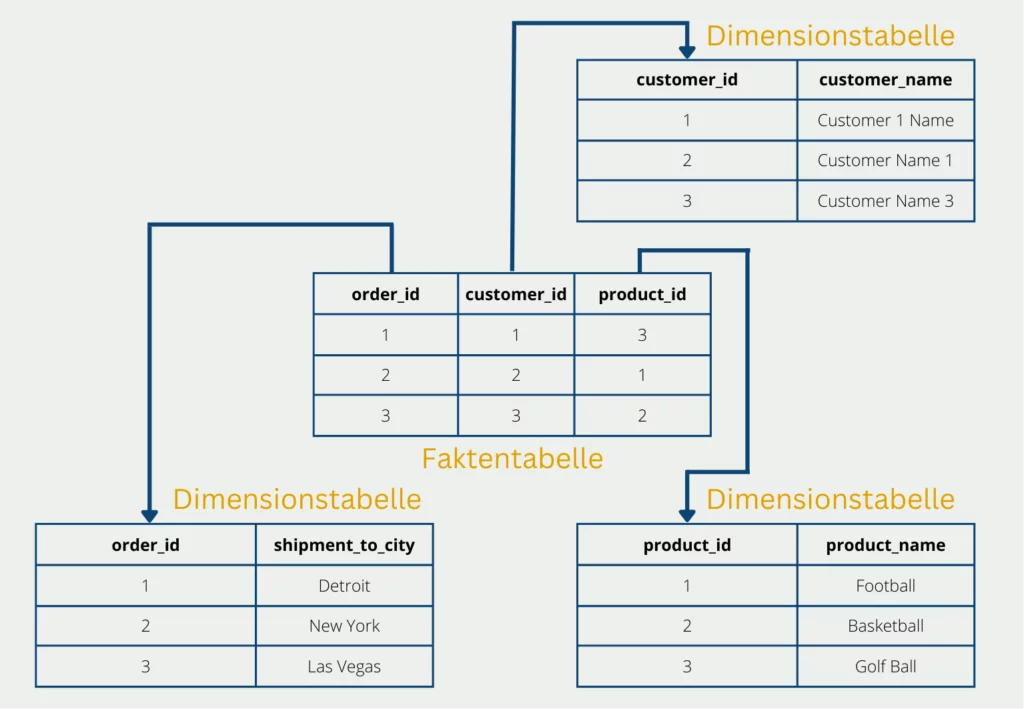
\includegraphics[scale=.26]{Bilder/SternSchemaDB.png}
\end{wrapfigure}

Der Primärschlüssel bezeichnet ein Attribut, das zur eindeutigen Identifikation einer Datenbankzeile verwendet werden kann. Dazu zählen beispielsweise die Rechnungsnummer zur Identifikation einer Rechnung oder die Ausweisnummer zur Identifikation einer Person.

\vspace{1em}

Konkret bedeutet dies in der Anwendung, dass \hl{alle Merkmale ausgelagert werden müssen, die nicht ausschließlich vom Primärschlüssel abhängig sind}. In der Praxis führt dies dann oft zu einem sogenannten Sternschema.


\paragraph{3. Normalform} Eine Relation liegt in der dritten Normalform vor, wenn sie in der ersten und zweiten Normalform vorliegt und \hl{keine transitiven Abhängigkeiten} bestehen.

Eine transitive Abhängigkeit liegt vor, wenn ein Attribut, welches kein Primärschlüssel ist, nicht nur von diesem abhängt, sondern auch von anderen Attributen.

Wenn wir in unserem Beispiel eine Tabelle haben, in der die Rechnungsnummer, die Produktnummer und der Preis gegeben ist, haben wir höchstwahrscheinlich eine transitive Abhängigkeit. \hl{Der Preis des Produktes hängt nämlich nicht wirklich von der Rechnungsnummer ab, sondern vielmehr von der Produktnummer}, da für jedes Produkt ein fester Preis definiert ist.

Diese Abhängigkeit kann man auflösen, indem man die Produkte in eine neue Tabelle auslagert und somit das Attribut Preis aus der ursprünglichen Tabelle rausfällt.

\subsubsection{Anomalien}
\label{sec:Anomalien}

Quelle: DatabaseCamp \cite{anomalien}

Anomalien in Datenbanken treten bei einer \hl{nicht existierenden oder fehlerhaften Normalisierung} auf.
Es existieren drei Arten von Datenbank-Anomalien, die Einfüge-Anomalie, die Änderungs-Anomalie und die Lösch-Anomalie.

In der Datenbanktentwicklung ist die Dritte Normalform oft ausreichend, um die perfekte Balance aus Redundanz, Performance und Flexibilität für eine Datenbank zu gewährleisten. Sie eliminiert auch die meisten Anomalien in einer Datenbank, aber nicht alle.

\paragraph{Einfügeanomalie} Bei einem fehlerhaften oder inkorrekten Datenbankdesign kann es bei der Einfüge-Anomalie passieren, dass Daten gar nicht in die Datenbank übernommen werden, wenn zum Beispiel der Primärschlüssel keinen Wert erhalten hat, oder eine \hl{unvollständigen Eingabe von Daten} zu Inkonsistenzen führt.

\paragraph{Änderungsanomalie} Bei der Änderungs-Anomalie, auch Update-Anomalie genannt, werden \hl{gleiche Attribute eines Datensatzes in einer Transaktion nicht automatisch geändert}. So entsteht eine Inkonsistenz der Daten.

\paragraph{Löschanomalie} Bei einer Löschanomalie kann es passieren, dass ein Benutzer einer Datenbank aktiv Informationen löschen will und damit indirekt, aufgrund des fehlerhaften Datenbankdesigns, \hl{andere zusammenhängende Informationen parallel mitlöscht}.

\subsection{SQL}
\label{sec:SQL}

Alle SQL-Komponenten für Abfragen siehe \referenz{sec:Datenbanken}.

\subsubsection{Projektion vs. Selektion}
\label{sec:ProjektionSelektion}

Quelle: Tino Hempel \cite{projektionSelektion}

\paragraph{Selektion} Bei der Selektion werden \hl{Zeilen aus einer Tabelle} ausgewählt, die bestimmten Eigenschaften genügen.

Aus der Tabelle Schüler sollen alle Zeilen selektiert werden, in denen der Name "Müller" steht. 
Die Selektion hat also die Form: $S_{Name} = _{'Mueller'}(Schueler)$

\vspace{1em}

\begin{minipage}{.45\textwidth}
	\begin{center}
		Schüler \\
		\vspace{1em}
		\bgroup
		\setlength{\tabcolsep}{1em}
		\def\arraystretch{1.5}
		\begin{tabular}{|c|l|l|}
			\hline
			\rowcolor{tableLightGray}\underline{SNr} & Vorname & Name \\
			\hline
			4711 & Paul & Müller \\
			\hline
			0815 & Erich & Schmidt \\
			\hline
			7472 & Sven & Lehmann \\
			\hline
			1234 & Olaf & Müller \\
			\hline
			2313 & Jürgen & Paulsen \\
			\hline
		\end{tabular}
		\egroup
	\end{center}
\end{minipage}
\hfill
\begin{minipage}{.45\textwidth}
	\begin{center}
		$S_{Name} = _{'Mueller'}(Schueler)$ \\
		\vspace{1em}
		\bgroup
		\setlength{\tabcolsep}{1em}
		\def\arraystretch{1.5}
		\begin{tabular}{|c|l|l|}
			\hline
			\rowcolor{tableLightGray}\underline{SNr} & Vorname & Name \\
			\hline
			12 & Paul & Müller \\
			\hline
			308 & Olaf & Müller \\
			\hline
		\end{tabular}
		\egroup
	\end{center}
\end{minipage}

\paragraph{Projektion} Bei der Projektion werden \hl{Spalten aus einer Tabelle} ausgewählt, die bestimmten Eigenschaften genügen.

Aus der Tabelle Schüler sollen alle Spalten mit dem Attribut 'Name' projiziert werden. 
Die Projektion hat also die Form: $P_{Name}(Schueler)$

\vspace{1em}

\begin{minipage}{.45\textwidth}
	\begin{center}
		Schüler \\
		\vspace{1em}
		\bgroup
		\setlength{\tabcolsep}{1em}
		\def\arraystretch{1.5}
		\begin{tabular}{|c|l|l|}
			\hline
			\rowcolor{tableLightGray}\underline{SNr} & Vorname & Name \\
			\hline
			4711 & Paul & Müller \\
			\hline
			0815 & Erich & Schmidt \\
			\hline
			7472 & Sven & Lehmann \\
			\hline
			1234 & Olaf & Müller \\
			\hline
			2313 & Jürgen & Paulsen \\
			\hline
		\end{tabular}
		\egroup
	\end{center}
\end{minipage}
\hfill
\begin{minipage}{.45\textwidth}
	\begin{center}
		$P_{Name}(Schueler)$ \\
		\vspace{1em}
		\bgroup
		\setlength{\tabcolsep}{1em}
		\def\arraystretch{1.5}
		\begin{tabular}{|l|}
			\hline
			\rowcolor{tableLightGray} Name \\
			\hline
			Müller \\
			\hline
			Schmidt \\
			\hline
			Lehmann \\
			\hline
			Müller \\
			\hline
			Paulsen \\
			\hline
		\end{tabular}
		\egroup
	\end{center}
\end{minipage}


\subsubsection{DDL, DML \& DCL}
\label{sec:DDLDMLDCL}

Quelle: GeeksforGeeks \cite{DDLDMLDCL}

\begin{enumerate}
	\item DDL - Data Definition Language
	\item DML - Data Manipulation Language
	\item DQL - Data Query Language
	\item DCL - Data Control Language
\end{enumerate}

\begin{center}
	\begin{tikzpicture}[
	item/.style={rectangle,draw,fill=blue!30, inner sep = 10},
	subitem/.style={rectangle,draw,fill=blue!20, inner sep = 8},
	grandchild/.style={grow=down,xshift=1em,anchor=west,
		edge from parent path={(\tikzparentnode.south) |- (\tikzchildnode.west)}},
	first/.style={level distance=6ex},
	second/.style={level distance=12ex},
	third/.style={level distance=18ex},
	forth/.style={level distance=24ex},
	level 1/.style={sibling distance=10em}]
	% Parents
	\coordinate
	node[item,anchor=east]{SQL Commands}
	child[grow=down,level distance=2.5ex]
	[edge from parent fork down]
	% Children and grandchildren
	child{node[item] {DDL}
		child[grandchild,first] {node[subitem]{CREATE}}
		child[grandchild,second] {node[subitem]{DROP}}
		child[grandchild,third] {node[subitem] {ALTER}}
		child[grandchild, forth] {node[subitem] {TRUNCATE}}}
	child{node[item] {DML}
		child[grandchild,first] {node[subitem]{INSERT}}
		child[grandchild,second] {node[subitem]{UPDATE}}
		child[grandchild,third] {node[subitem]{DELETE}}}
	child {node[item]{DQL}
		child[grandchild,first] {node[subitem]{SELECT}}}
	child {node[item]{DCL}
		child[grandchild,first] {node[subitem]{GRANT}}
		child[grandchild,second] {node[subitem]{REVOKE}}};
\end{tikzpicture}
\end{center}

\subsubsection{CRUD}
\label{sec:CRUD}

Quelle: sqlshack.com \cite{crud}

\paragraph{C} refers to CREATE aka add, insert. In this operation, it is expected to insert a new record using the SQL insert statement. SQL uses \hl{INSERT INTO} statement to create new records within the table.

\begin{lstlisting}[language=SQL]
	INSERT INTO <tablename> (column1,column2,...) 
	VALUES(value1,value2,...),( value1,value2,...), (value1,value2,...)...
\end{lstlisting}

\begin{lstlisting}[language=SQL]
	INSERT INTO dbo.Demo
	(id, name)
	VALUES
	(2, 'Jayaram'),
	(3, 'Pravitha');
\end{lstlisting}

\paragraph{R} refers to SELECT (data retrieval) operation. The word ‘read’ retrieves data or record-set from a listed table(s). SQL uses the SELECT command to retrieve the data.

\begin{lstlisting}[language=SQL]
	SELECT * FROM <TableName>;
\end{lstlisting}

\paragraph{U} refers to Update operation. Using the Update keyword, SQL brings a change to an existing record(s) of the table. When performing an update, you’ll need to define the target table and the columns that need to update along with the associated values, and you may also need to know which rows need to be updated. In general, you want to limit the number of rows in order to avoid lock escalation and concurrency issues.

\begin{lstlisting}[language=SQL]
	UPDATE <TableName>
	SET Column1=Value1, Column2=Value2,...
	WHERE <Expression>
\end{lstlisting}

\paragraph{D} refers to removing a record from a table. SQL uses the SQL DELETE command to delete the record(s) from the table.

\begin{lstlisting}[language=SQL]
	DELETE FROM <TableName>
	WHERE <Expression>
\end{lstlisting}

\subsubsection{Subqueries}
\label{sec:Subquery}



\subsubsection{Aggregatfunktionen}
\label{sec:Aggregatfunktionen}

\subsubsection{Schnitt-, Vereinigungs- und Differenzmenge}
\label{sec:SchnittVereinigungsDifferenzmenge}

\subsubsection{SQL Injection}
\label{sec:SQLInjection}

